%!TEX TS-program = xelatex

\documentclass[t]{beamer}

\usetheme{Hannover}
\usecolortheme{rose}

%%% Работа с русским языком
\usepackage[english,russian]{babel}   %% загружает пакет многоязыковой вёрстки
\usepackage{fontspec,xltxtra,xunicode}      %% подготавливает загрузку шрифтов Open Type, True Type и др.
%\defaultfontfeatures{Ligatures={TeX},Renderer=Basic}  %% свойства шрифтов по умолчанию
\setmainfont[Ligatures={TeX,Historic},
SmallCapsFont={Brill},
SmallCapsFeatures={Letters=SmallCaps}]{Brill} %% задаёт основной шрифт документа
\setsansfont{Brill}                    %% задаёт шрифт без засечек
\setmonofont[Ligatures=NoCommon]{DejaVu Sans}
\newfontfamily\SYM{Brill}
\usepackage{indentfirst}
%%% Дополнительная работа с математикой
\usepackage{amsmath,amsfonts,amssymb,amsthm,mathtools} % AMS
\usepackage{icomma} % "Умная" запятая: $0,2$ --- число, $0, 2$ --- перечисление

%%% Работа с картинками
\usepackage{wrapfig} % Обтекание рисунков текстом
\usepackage{rotating}
\usepackage{fixltx2e}
\usepackage{hhline}
\usepackage{lscape}

%%% Работа с таблицами
\usepackage{array,tabularx,tabulary,booktabs} % Дополнительная работа с таблицами
\usepackage{longtable}  % Длинные таблицы
\usepackage{multirow} % Слияние строк в таблице

\usepackage{multicol} % Несколько колонок

%%% Страница
%\usepackage{fancyhdr} % Колонтитулы
% 	\pagestyle{fancy}
 	%\renewcommand{\headrulewidth}{0pt}  % Толщина линейки, отчеркивающей верхний колонтитул
% 	\lfoot{Нижний левый}
% 	\rfoot{Нижний правый}
% 	\rhead{Верхний правый}
% 	\chead{Верхний в центре}
% 	\lhead{Верхний левый}
%	\cfoot{Нижний в центре} % По умолчанию здесь номер страницы

\usepackage{setspace} % Интерлиньяж
%\onehalfspacing % Интерлиньяж 1.5
%\doublespacing % Интерлиньяж 2
\singlespacing % Интерлиньяж 1

\usepackage{subfig} % подкартинки
\usepackage{lastpage} % Узнать, сколько всего страниц в документе.
\usepackage{soul} % Модификаторы начертания
\usepackage{bbding}
\usepackage{hyperref}
\usepackage{tikz} % Работа с графикой
\usepackage{pgfplots}
\usepackage{pgfplotstable}
\usepackage{verbatim}

\usepackage{attachfile2}
 \attachfilesetup{appearance=true,
color=0 0 0
 }
\usepackage{alltt}

%%% Лингвистические пакеты
%\usepackage{savetrees} % пакет, который экономит место
\usepackage{forest} % для рисования деревьев
\usepackage{vowel} % для рисования трапеций гласных
\usepackage{natbib}
\bibpunct[: ]{[}{]}{;}{a}{}{,}
\usepackage[nogroupskip,nopostdot, nonumberlist]{glossaries}
%\usepackage{glossary-mcols} 
%\setglossarystyle{mcolindex}
\usepackage{philex} % пакет для примеров
\newcommand{\mytem}{\item[$\circ$]}
\addto\captionsrussian{
\renewcommand{\refname}{}}

\newcommand{\apostrophe}{\XeTeXglyph\XeTeXcharglyph"0027\relax}
\usetikzlibrary{patterns}

\usepackage{ulem}
\usepackage{subfig}
\setbeamercolor{alerted text}{fg=red!13!blue}
\setbeamersize{text margin left=4mm,text margin right=1mm} 
\setbeamertemplate{navigation symbols}{
	\usebeamerfont{footline}%
    \usebeamercolor[fg]{footline}%
    \hspace{1em}%
    {{\small презентация доступна: \href{http://goo.gl/ZNJ0Gj}{\textbf{http://goo.gl/ZNJ0Gj}}}
    \hspace{4.3cm}
    \insertframenumber/\inserttotalframenumber\vspace{0.5mm}}}
\newcommand{\mcrot}[4]{\multicolumn{#1}{#2}{\rlap{\rotatebox{#3}{#4}~}}} 
% начало
\title[]{Логистическая регрессия}
\author[]{Г. Мороз}
\date{}
\begin{document}
\frame{\titlepage}
\section{основы}
\begin{frame}{Логистическая регрессия}
Логистическая регрессия или логит-регрессия (logistic regression, logit regression) была описана в работе \citep{cox58} и применяется в случаях, когда зависимая переменная принимает два значения а предикторы могут быть как числовыми, так и категориальными.
\end{frame}
\begin{frame}{шансы, натуральный логарифм}
\vspace{-2mm}
Мы хотим чего-то такого:
$$\underbrace{y}_{[-\infty, +\infty]}=\underbrace{\mbox{β}_0+\mbox{β}_1\cdot x_1+\mbox{β}_2\cdot x_2 + \dots +\mbox{β}_k\cdot x_k +\mbox{ε}_i}_{[-\infty, +\infty]}$$
Вероятность — (в классической статистике) отношение количества успехов к общему числу событий:
$$p = \frac{\mbox{\# успехов}}{\mbox{\# неудач} + \mbox{\# успехов}}, \mbox{область значений: }[0, 1]$$
Шансы — отношение количества успехов к количеству неудач:
$$odds = \frac{p}{1-p} = \frac{\mbox{p(успеха)}}{\mbox{p(неудачи)}}, \mbox{область значений: }[0, +\infty]$$
Натуральный логарифм шансов:
$$log(odds), \mbox{область значений: }[-\infty, +\infty]$$
\end{frame}
\begin{frame}{вероятность $\longleftrightarrow$ логарифм шансов}
\begin{columns}[T] 
\begin{column}{.48\textwidth}
\begin{tabular}{c|c|c|c|c}
\# у & \# н & $p$ & $odds$ & $log(odds)$ \\ \hline
1 & 9 & 0.1 & 0.11 & -2.20 \\ \hline
2 & 8 & 0.2 & 0.25 & -1.39 \\ \hline
3 & 7 & 0.3 & 0.43 & -0.85 \\ \hline
4 & 6 & 0.4 & 0.67 & -0.41 \\ \hline
5 & 5 & 0.5 & 1& 0 \\ \hline
6 & 4 & 0.6 & 1.5 & 0.41 \\ \hline
7 & 3 & 0.7 & 2.33 & 0.85 \\ \hline
8 & 2 & 0.8 & 4 & 1.39 \\ \hline
9 & 1 & 0.9 & 9 & 2.20 \\
\end{tabular}
\end{column}
\hfill
\begin{column}{.48\textwidth}
\scriptsize
\begin{alltt}
~~~~~a <- 1:9\\
~~~~~b <- 9:1\\
~~~~~p <- a/(b+a)\\
~~~~~\alert{lo <- log(p/(1-p))}\bigskip\\
~~~~~\alert{p <- exp(lo)/(1 + exp(lo))}
\end{alltt}
\normalsize
\end{column}
\end{columns}
\end{frame}
\begin{frame}{сигмоида}
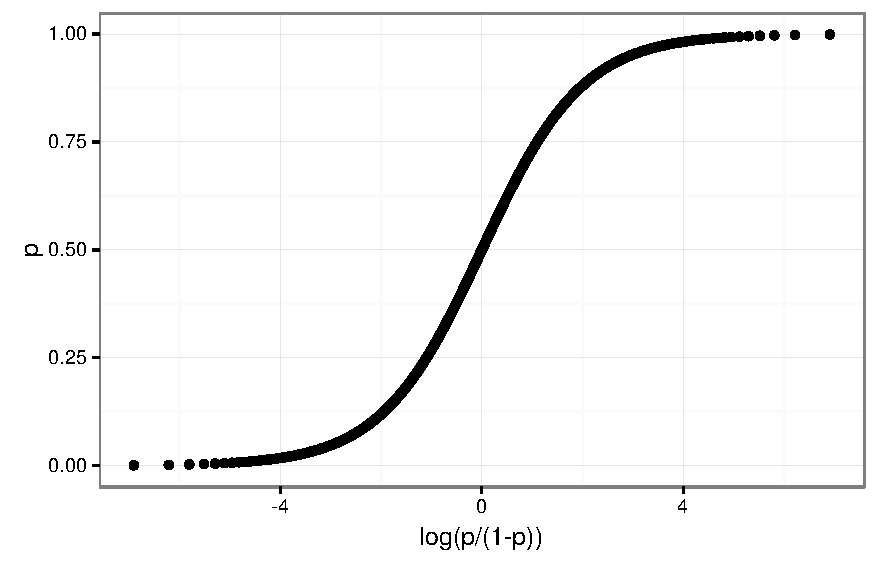
\includegraphics[width=\linewidth]{sigmoid.pdf}
\end{frame}
\section{модели}
\begin{frame}{Задача 1}
Проанализируем \href{http://goo.gl/0btfKa}{\alert{данные}}, содержащих выборку языков с указанием количества согласных и наличия в данном языке абруптивных согласных. На графике представлен результат (можно посмотреть \href{http://goo.gl/JgrU6g}{\alert{более интерактивный вариант}}):\\
\vfill
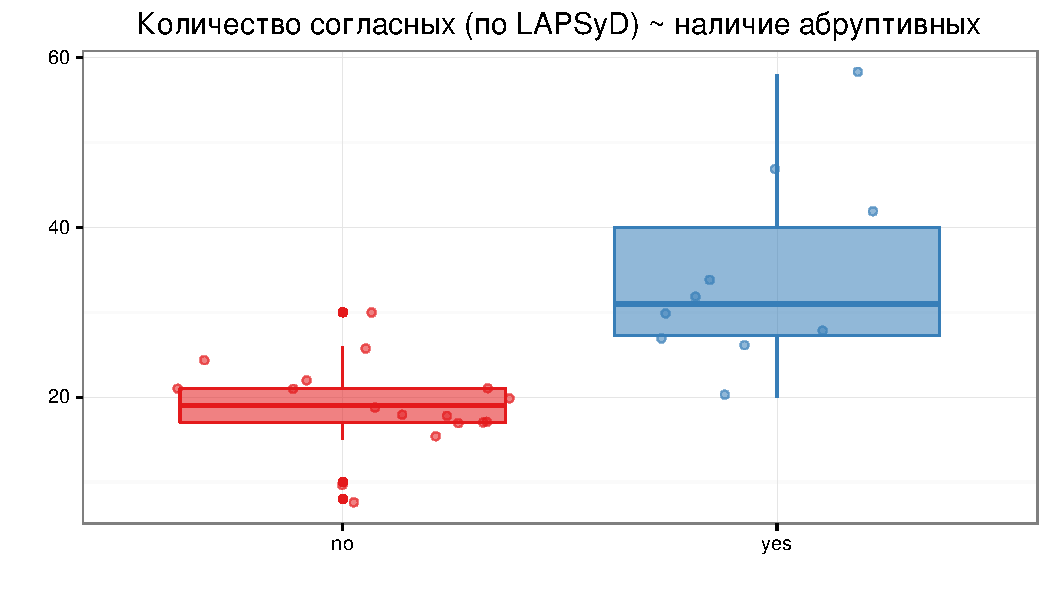
\includegraphics[width=0.95\linewidth]{ejectives.pdf}
\end{frame}
\subsection{без предикторов}
\begin{frame}{Модель без предикторов}
\vspace{-5mm}
\scriptsize
\begin{alltt}
df <- read.csv("http://goo.gl/0btfKa")\\
fit1 <- \alert{glm(ejectives \textasciitilde 1}, data = df, \alert{family = "binomial")} \hfill \# логит-регрессия\\
summary(fit1)\medskip\\
Call:\\
glm(formula = ejectives \textasciitilde 1, family = "binomial"{}, data = df) \hfill \# \alert{формула}\medskip\\
Deviance Residuals: \hfill \# \alert{распределение остатков} \\
\begin{tabular}{rrrrr}
    Min   &    1Q &  Median  &     3Q &     Max  \\
-0.9619  & -0.9619 &  -0.9619 &  1.4094 &  1.4094\\  
\end{tabular}
\medskip\\
Coefficients: \hfill \# \alert{коэфициенты модели}\\
\begin{tabular}{rrrrrr}
    &       \alert{Estimate} & Std. Error & z value & Pr(>|z|)&\\
\alert{(Intercept)} &  \alert{-0.5306}  &   0.3985 &  -1.331  &  0.183 & \hfill \# \alert{β$_0$}\\
\end{tabular} \medskip\\
(Dispersion parameter for binomial family taken to be 1)\medskip\\
    Null deviance: 35.594  on 26  degrees of freedom\\
Residual deviance: 35.594  on 26  degrees of freedom\\
AIC: 37.594 \hfill \# \alert{критерий Акаике}\medskip\\
Number of Fisher Scoring iterations: 4\\
\rule{\linewidth}{0.4pt}
\alert{table(df\$ejectives)} \hfill \# \alert{а сколько у нас языков с абруптивами?}\\
\begin{tabular}{rr}
no & yes\\ 
 17  & 10 \\
\end{tabular} \\
\alert{log(10/17)}\\
-0.5306283 \hfill \# \alert{так вот как получен коэфициент β$_0$…}
\end{alltt}
\normalsize
\end{frame}
\subsection{числовой предиктор}
\begin{frame}{Модель с числовым предиктором}
\vspace{-5mm}
\scriptsize
\begin{alltt}
df <- read.csv("http://goo.gl/0btfKa")\\
fit2 <- \alert{glm(ejectives \textasciitilde n.cons.lapsyd}, data = df, \alert{family = "binomial")} \\
summary(fit2)\medskip\\
Call:\\
glm(formula = ejectives \textasciitilde n.cons.lapsyd, family = "binomial"{},  data = df)\medskip\\
Deviance Residuals: \hfill \# \alert{распределение остатков} \\
\begin{tabular}{rrrrr}
    Min   &    1Q &  Median  &     3Q &     Max  \\
-1.8317  & -0.4742 &  -0.2481 &  0.1914  & 2.1997 \\
\end{tabular}
\medskip\\
Coefficients: \hfill \# \alert{коэфициенты модели}\\
\begin{tabular}{rrrrrrr}
    &       \alert{Estimate} & Std. Error & z value & Pr(>|z|)& &\\
\alert{(Intercept)} &  \alert{-9.9204}  &  3.7699 &  -2.631   & 0.0085 &**&\hfill \# \alert{β$_0$}\\
\alert{n.cons.lapsyd}  & \alert{0.3797} &  0.1495  &  2.540 &  0.0111 & * & \hfill \# \alert{β$_1$}
\end{tabular} \medskip\\
Signif. codes:  0 ‘***’ 0.001 ‘**’ 0.01 ‘*’ 0.05 ‘.’ 0.1 ‘ ’ 1 \medskip\\
(Dispersion parameter for binomial family taken to be 1) \medskip\\
Null deviance: 35.594  on 26  degrees of freedom\\
Residual deviance: 16.202  on 25  degrees of freedom\\
AIC: 20.202 \hfill \# \alert{критерий Акаике}\medskip\\
Number of Fisher Scoring iterations: 6
\end{alltt}
\normalsize
\end{frame}
\begin{frame}{Визуализация: ggplot2}
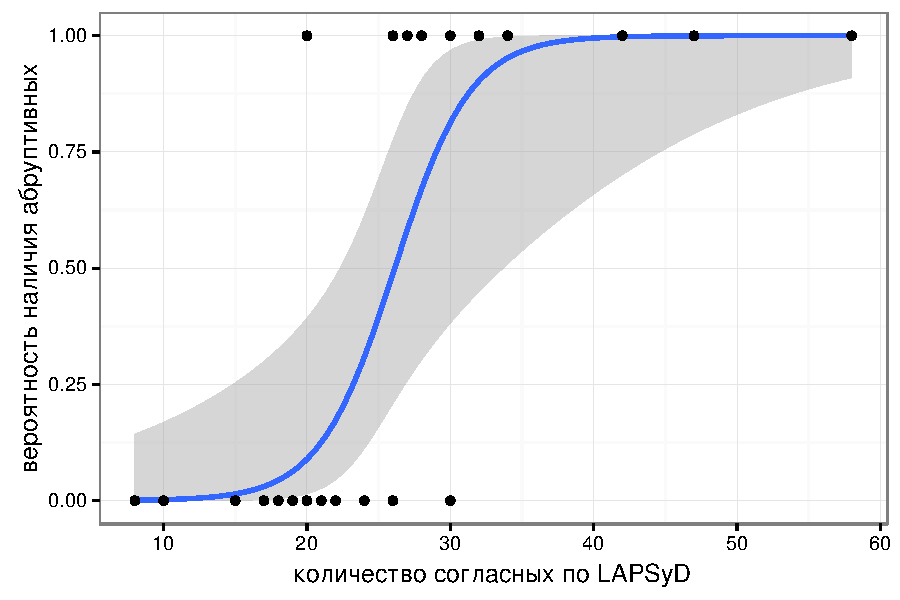
\includegraphics[width=\linewidth]{ejectivessigmoid.pdf}
\end{frame}
\begin{frame}{Визуализация: ggplot2}
\scriptsize
\begin{alltt}
df <- read.csv("http://goo.gl/0btfKa")\medskip\\
\alert{str(df)}\\
'data.frame':	27 obs. of  3 variables:\\
\$ name: \alert{Factor} w/ 27 levels "Abkhaz"{},"Amharic"{},..: 25 15 22 16 24 19 14 7 ...\\
 \$ n.cons.lapsyd: \alert{int}  24 21 21 22 21 20 19 18 15 17 ...\\
\$ ejectives: \alert{Factor} w/ 2 levels "no"{},"yes"{}: 1 1 1 1 1 1 1 1 1 1 ...\medskip\\
\# Нужно переделать значения переменной ejectives в 0 и 1\\
df\$ejectives.value <- \alert{as.numeric(}df\$ejectives\alert{) - 1}\medskip\\
library(ggplot2)\\
ggplot(data = df, aes(x = n.cons.lapsyd, y = ejectives.value))+\\
~~\alert{geom\_smooth(method = "glm"{}, method.args = list(family = "binomial"))} +\\
~~geom\_point() \bigskip\\
\end{alltt}
\normalsize
Чтобы убрать доверительный интервал, можно добавить аргумент \scriptsize\alert{\verb"ls~=~F"}\normalsize\ в функцию \scriptsize\verb"geom\_smooth()"\normalsize.
\end{frame}
\begin{frame}{Интерпретация}
Какова вероятность по нашим данным, что в языке с 29 согласными есть абруптивные звуки?
$$\log(odds) \mbox{ или} \log\left(\frac{p}{1-p}\right) = \mbox{β}_0+\mbox{β}_1\times \mbox{n.cons.lapsyd}$$
$$ p = \frac{e^{\log(odds)}}{1+e^{\log(odds)}}$$
\vfill
$$\mbox{β}_0+\mbox{β}_1\times \mbox{n.cons.lapsyd} =  -9.9204+0.3797 \times 29 = 1.0909$$
$$\frac{e^{\log(odds)}}{1+e^{\log(odds)}} = \frac{e^{1.0909}}{1+e^{1.0909}} = 0.7485512$$
Т. е. в соответствии с нашими данными, вероятность, что в языке с 29 согласными есть абруптивные звуки примерно 3 к 1 или 0.75.
\end{frame}
\begin{frame}{Предсказания, на основе модели}
Неужели необходимо помнить все эти формулы?
\scriptsize
\begin{alltt}
new <- data.frame(\alert{n.cons.lapsyd = 29})\\
\alert{predict(fit2, new, type="response")}\\
\begin{tabular}{r}
        1 \\
0.7485964 \\
\end{tabular}
\end{alltt}
\normalsize
Функция \scriptsize\verb"predict()"\normalsize\ принимает на вход построенную модель (не обязательно логистическую) и датафрейм со столбцами, использованными для построения модели. Естественно, значений может быть несколько.
\scriptsize
\begin{alltt}
new <- data.frame(n.cons.lapsyd = \alert{27:31})\\
predict(fit2, new, type="response")\\
\begin{tabular}{rrrrrr}
        1  & 2 & 3& 4 & 5\\
0.5821783 & 0.6707173 & 0.7485964 & 0.8131865 & 0.8641927\\
\end{tabular}
\end{alltt}
\normalsize
Чтобы получить не вероятности, а значение шансов (\textit{odds}), следует в аргументе \scriptsize\verb"type"\normalsize\ указать значение \scriptsize\verb"link"\normalsize\ (это значение по умолчанию).
\scriptsize
\begin{alltt}
new <- data.frame(n.cons.lapsyd = 27:31)\\
predict(fit2, new, \alert{type="link"})\\
\begin{tabular}{rrrrrr}
        1  & 2 & 3& 4 & 5\\
0.3317220& 0.7114312 & 1.0911404 & 1.4708496 & 1.8505588 \\
\end{tabular}
\end{alltt}
\normalsize
\end{frame}
\begin{frame}{Доверительные интервалы для наблюдений}
Можно построить доверительный интервал для каждого наблюдения:
\scriptsize
\begin{alltt}
df <- read.csv("http://goo.gl/0btfKa")\\
fit2 <- \alert{glm(ejectives \textasciitilde n.cons.lapsyd}, data = df, \alert{family = "binomial")}\medskip\\
pred <- predict(fit2, type="response"{}, se.fit = T)\\
df <- cbind.data.frame(df, fit = pred\$fit, se.fit = pred\$se.fit)\\
head(df)\\
\begin{tabular}{rrrrrr}
&        name & n.cons.lapsyd & ejectives  &      \alert{fit}  &   \alert{se.fit}\\
1  &  Turkish        &    24    &    no   &  \alert{0.30844363} & \alert{0.13769764}\\
2 &    Korean      &      21     &   no & \alert{0.12493187} & \alert{0.09358363}\\
3    &   Tiwi        &    21      &  no & \alert{0.12493187} & \alert{0.09358363}\\
4   &  Kpelle    &        22     &   no & \alert{0.17266963} & \alert{0.10904915}\\
5      & Tulu         &   21   &     no & \alert{0.12493187} & \alert{0.09358363}\\
&&&& \multicolumn{1}{c}{\alert{↑}} & \multicolumn{1}{c}{\alert{↑}} \\
&&&& \alert{вероятности} & \alert{довер. инт.} \\
\end{tabular}
\end{alltt}
\end{frame}
\begin{frame}{Визуализация: ggplot2}
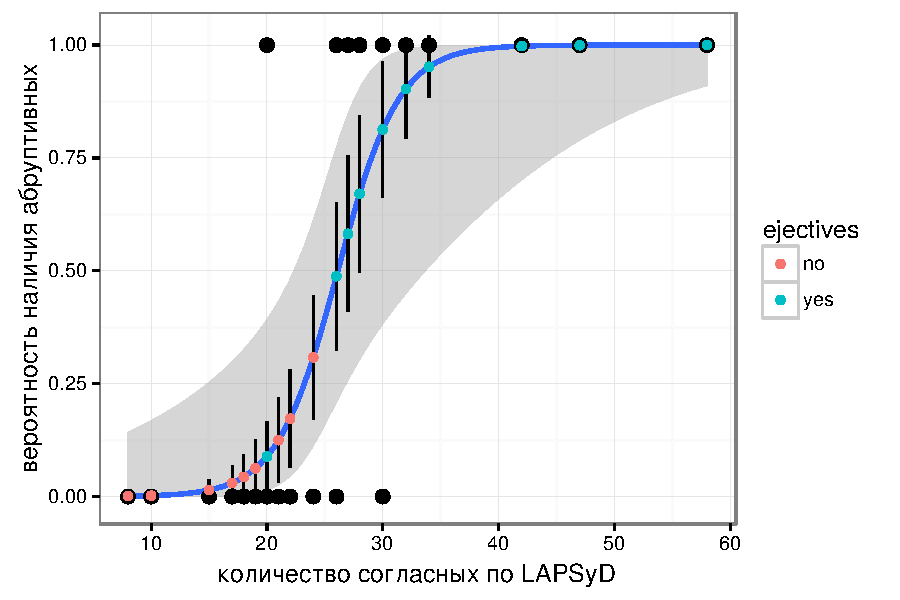
\includegraphics[width=\linewidth]{logitse.pdf}
\end{frame}
\begin{frame}{Визуализация: ggplot2}
\scriptsize
\begin{alltt}
df <- read.csv("http://goo.gl/0btfKa")\\
fit2 <- \alert{glm(ejectives \textasciitilde n.cons.lapsyd}, data = df, \alert{family = "binomial")}\medskip\\
pred <- predict(fit2, type="response"{}, se.fit = T) \hfill \# вероятности и CI\\
df <- cbind.data.frame(df, fit = pred\$fit, se.fit = pred\$se.fit)\medskip\\
\# Нужно переделать значения переменной ejectives в 0 и 1\\
df\$ejectives.value <- \alert{as.numeric(}df\$ejectives\alert{) - 1}\medskip\\
library(ggplot2)\\
ggplot(data = df, aes(x = n.cons.lapsyd, y = ejectives.value))+\\
~~~\hfill \# сигмоида \\
~~~geom\_smooth(method = "glm"{}, method.args = list(family = "binomial"))+\\
~~~geom\_point() + \hfill \# наблюдения\\
\alert{~~~geom\_pointrange(aes(x = n.cons.lapsyd, \hfill \# CI для вероятностей\\
~~~~~~~~~~~~~~~~~~~~~~~~~~~~~~~~~~~~~~~~~~~~~~~~~~~~~~~~~~~~ymin = fit - se.fit, ymax = fit + se.fit))+\\
\hfill \# вероятности\\
~~~geom\_point(aes(x = n.cons.lapsyd, y = fit, colour = ejectives))} \\
\end{alltt}
\normalsize
\end{frame}
\begin{frame}{Визуализация: ggplot2}
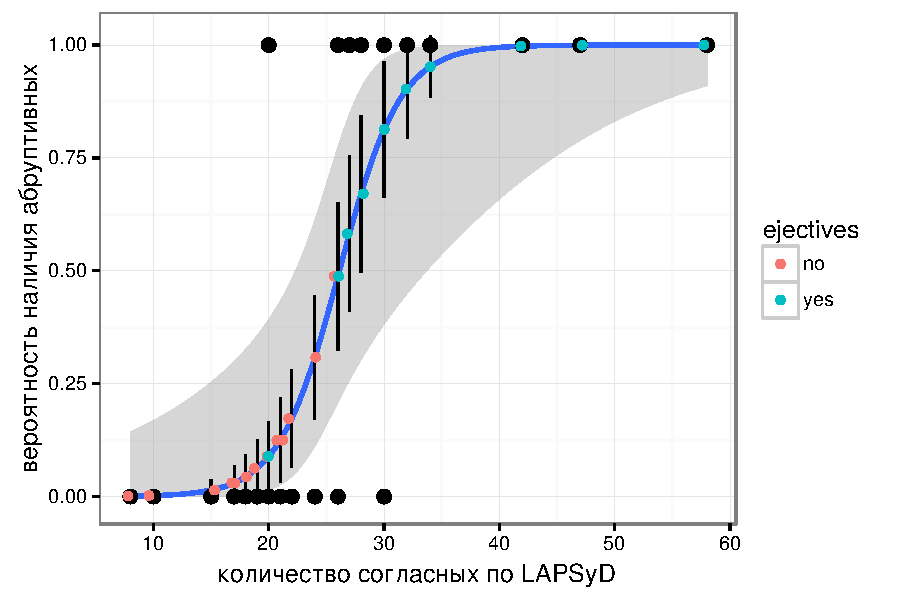
\includegraphics[width=\linewidth]{logitsejitter.pdf}
\end{frame}
\begin{frame}{Визуализация: ggplot2}
\scriptsize
\begin{alltt}
df <- read.csv("http://goo.gl/0btfKa")\\
fit2 <- \alert{glm(ejectives \textasciitilde n.cons.lapsyd}, data = df, \alert{family = "binomial")}\medskip\\
pred <- predict(fit2, type="response"{}, se.fit = T) \hfill \# вероятности и CI\\
df <- cbind.data.frame(df, fit = pred\$fit, se.fit = pred\$se.fit)\medskip\\
\# Нужно переделать значения переменной ejectives в 0 и 1\\
df\$ejectives.value <- \alert{as.numeric(}df\$ejectives\alert{) - 1}\medskip\\
library(ggplot2)\\
ggplot(data = df, aes(x = n.cons.lapsyd, y = ejectives.value))+\\
~~~\hfill \# сигмоида \\
~~~geom\_smooth(method = "glm"{}, method.args = list(family = "binomial"))+\\
~~~geom\_point() + \hfill \# наблюдения\\
~~~geom\_pointrange(aes(x = n.cons.lapsyd, \hfill \# CI для вероятностей\\
~~~~~~~~~~~~~~~~~~~~~~~~~~~~~~~~~~~~~~~~~~~~~~~~~~~~~~~~~~~~ymin = fit - se.fit, ymax = fit + se.fit))+\\
\hfill \# вероятности\\
~~~geom\_\alert{jitter}(aes(x = n.cons.lapsyd, y = fit, colour = ejectives)) \\
\end{alltt}
\normalsize
\end{frame}
\subsection{категориальный пред.}
\begin{frame}{Задача 2}
В работе [Coates, Leech 1980: 31] приводятся результаты исследования значений модальных глаголов (\textit{must}, \textit{have to}) в британском и американском английском. Авторы выделяют два значения в употреблении модальных глаголов буквальное (\textit{you must read it}) и эпистемическое (\textit{you must be kidding}). \href{http://goo.gl/4iEt4j}{\alert{Данные}} основаны на \href{http://files.eric.ed.gov/fulltext/ED202217.pdf}{\alert{работе Coates, J., Leech, G. (1980) The Meanings of the Modals in British and American English}}.\\
\vfill
Для начала попробуем предсказать какой будет выбираться глагол на основе значения.
\end{frame}
\begin{frame}{Модель с категориальным предиктором}
\vspace{-5mm}
\scriptsize
\begin{alltt}
df <- read.csv("http://goo.gl/4iEt4j")\\
fit3 <- \alert{glm(word \textasciitilde meaning}, data = df, \alert{family = "binomial")} \\
summary(fit3)\medskip\\
Call:\\
glm(formula = word \textasciitilde meaning, family = "binomial",  data = df)\medskip\\
Deviance Residuals: \hfill \# \alert{распределение остатков} \\
\begin{tabular}{rrrrr}
    Min   &    1Q &  Median  &     3Q &     Max  \\
-2.229  & -1.028 &  -1.028 &  1.334 &  1.334 \\
\end{tabular}
\medskip\\
Coefficients: \hfill \# \alert{коэфициенты модели}\\
\begin{tabular}{rrrrrrr}
    &       \alert{Estimate} & Std. Error & z value & Pr(>|z|)& &\\
\alert{(Intercept)} & \alert{2.3979}    & 0.3148  &  7.618 & 2.59e-14 & ***&\hfill \# \alert{β$_0$}\\
\alert{meaning}  & \alert{-2.7595}     & 0.3236 &  -8.529  & < 2e-16 & *** & \hfill \# \alert{β$_1$}
\end{tabular} \medskip\\
Signif. codes:  0 ‘***’ 0.001 ‘**’ 0.01 ‘*’ 0.05 ‘.’ 0.1 ‘ ’ 1 \medskip\\
(Dispersion parameter for binomial family taken to be 1) \medskip\\
Null deviance: 1205.5  on 869  degrees of freedom\\
Residual deviance: 1075.1  on 868  degrees of freedom\\
AIC: 1079.1 \hfill \# \alert{критерий Акаике}\medskip\\
Number of Fisher Scoring iterations: 4
\end{alltt}
\normalsize
\end{frame}
\begin{frame}{Как были получены эти значения?}
\scriptsize
\begin{alltt}
table(df\$meaning, df\$word) \hfill \# построим матрицу сопряженности
\begin{tabular}{rrr}
       &   epistemic & root\\
  have to   &     11 & 435\\
  must        &  121 & 303\\
  \end{tabular}
\medskip\\
fit3 <- \alert{glm(word \textasciitilde meaning}, data = df, \alert{family = "binomial")} \\
fit3\$coefficients\\
\begin{tabular}{rr}
(Intercept) & meaningroot \\
   2.397895 &  -2.759508 \\
\end{tabular}
\end{alltt}
\normalsize
$$\log(odds)  = 2.397895 + (-2.759508) \times \mbox{meaningroot}$$
В интерсепте логарифм шансов случаев с эпистемической модальностью
$$\log\left(\frac{121}{11}\right) = 2.397895$$
Второй коэффициент в сумме с интерсептом составляют логарифм шансов случаев с прямым значением
$$\log\left(\frac{303}{435}\right) = -0.3616132 = 2.397895 + (-2.759508)$$
\end{frame}
\begin{frame}{Доверительный интервал для коэффициентов}
Для коэффициентов модели можно посчитать доверительный интервал:
\scriptsize
\begin{alltt}
df <- read.csv("http://goo.gl/4iEt4j")\\
fit3 <- \alert{glm(word \textasciitilde\ meaning}, data = df, \alert{family = "binomial")}\medskip\\
\alert{confint(fit3)}\\
Waiting for profiling to be done…\\
\begin{tabular}{rrr}
    &   2.5 \%  &  97.5 \% \\
(Intercept) & 1.828070 &  3.074627\\
meaningroot & -3.450629  & -2.169762\\
\end{tabular}
\end{alltt}
\normalsize
\end{frame}
\section{синтаксическая заметка}
\begin{frame}{Aspects \sout{of the Theory} of Syntax}
\begin{itemize}
\mytem $y=\mbox{β}_0+\mbox{β}_1\cdot x_1 +\mbox{ε}_i$ \hfill обычная формула\\
\scriptsize
\begin{alltt}
\alert{y\textasciitilde x}
\end{alltt}
\normalsize
\mytem $y=\mbox{β}_0+\mbox{β}_1\cdot x_1 +\mbox{β}_2\cdot x_2 +\mbox{ε}_i$ \hfill обычная формула\\
\scriptsize
\begin{alltt}
\alert{y\textasciitilde x + z}
\end{alltt}
\normalsize
\mytem $y=\mbox{β}_0+\mbox{β}_1\cdot x_2\cdot x_1 +\mbox{ε}_i$ \hfill только взаимодействие\\
\scriptsize
\begin{alltt}
\alert{y\textasciitilde x:z}
\end{alltt}
\normalsize
\mytem $y=\mbox{β}_0+\mbox{β}_1\cdot x_1 +\mbox{β}_2\cdot x_2 +\mbox{β}_3\cdot x_2\cdot x_1 +\mbox{ε}_i$ \hfill с взаимодействием\\
\scriptsize
\begin{alltt}
\alert{y\textasciitilde x*z\hfill }
\end{alltt}
\normalsize
\mytem $y=\mbox{β}_0 +\mbox{ε}_i$ \hfill формула без предикторов\\
\scriptsize
\begin{alltt}
\alert{y\textasciitilde 1}
\end{alltt}
\normalsize
\mytem $y=\mbox{β}_1\cdot x_1 +\mbox{ε}_i$ \hfill формула без свободного члена\\
\scriptsize
\begin{alltt}
\alert{y\textasciitilde x - 1}
\end{alltt}
\normalsize
\mytem $y=\mbox{β}_0+\mbox{β}_1\cdot x_1+\mbox{β}_2\cdot x_2 + \dots +\mbox{β}_k\cdot x_k +\mbox{ε}_i$ \hfill все предикторы\\
\scriptsize
\begin{alltt}
\alert{y\textasciitilde \textbf{.}}
\end{alltt}
\normalsize
\end{itemize}
\scriptsize
\begin{alltt}

\end{alltt}
\normalsize
\end{frame}

\begin{frame}
{\huge Спасибо за внимание\bigskip\\
\normalsize Пишите письма\\
agricolamz@gmail.com
\vspace{-130pt}}
\end{frame}
\begin{frame}{Список литературы}
\footnotesize
\bibliographystyle{chicago}
\bibliography{bibliography}
\end{frame}
\end{document}
